\documentclass[paper=a4]{jlreq}
\usepackage{amsmath,amssymb}
\usepackage{bm}
\usepackage{here}
\usepackage{graphicx}
\usepackage{hyperref}
\usepackage{physics}
\usepackage{subcaption}
\usepackage{tikz}
\usepackage{xcolor}

\definecolor{cud_red}{RGB}{255,75,0}
\definecolor{cud_green}{RGB}{3,175,122}
\definecolor{cud_blue}{RGB}{0,90,255}
\definecolor{cud_sky}{RGB}{77,196,255}
\usetikzlibrary{intersections, calc, arrows}
\hypersetup{
    colorlinks=true,
    linkcolor=cud_blue,
    citecolor=cud_green,
    filecolor=cud_blue,      
    urlcolor=cud_green,
}

\begin{document}
\title{2次元FEMのメモ}
\author{きゅーしす}
\date{}
\maketitle

文献\cite{Larson2013}を参考にして2次元有限要素法の
境界値問題を定式化して解く.

\section{有限要素の簡単な説明}
はじめに, 読者のみなさんに有限要素法を解説したいと思います。
有限要素法 (Finite Element Method)とは微分方程式を積分で定式化した上で
重み付き残差法を用いて近似解を求める手法です。

何を言っているのかわからない人が多いと思いますので1次元の常微分方程式を
例に有限要素法の簡単な説明をします。
解く問題は
\begin{align}
    \frac{\mathrm{d}^2u}{\mathrm{d}^2x} +f &=0 \label{eq:ode} \\
    u(0) = u(L) &= 0 \label{eq:ode:bc}
\end{align}

\section{Dirichlet問題の有限要素解析}
以下の偏微分方程式の境界値問題を考える.
以下の条件の未知関数$u$を求める. 
ここで$\Omega$は単連結な領域で$f$と$g_D$は既知の関数であるものとする.
\begin{alignat}{4}
    \nabla^2 u + f &= 0 &\quad& \mathrm{in}\, \Omega \label{eq:poisson}\\
    u &= g_D &\quad& \mathrm{on}\, \partial\Omega \label{eq:dirichlet_bc}
\end{alignat}
重み関数$v$を$f = -\nabla^2 u$に掛けて積分し, 以下の式を得る.
\begin{align}
    \begin{split}
        \int_\Omega fv\dd{V} &= -\int_\Omega \nabla^2 u \dd{V} \\
        &= \int_\Omega \nabla u\cdot \nabla v \dd{V} 
        + \int_{\partial\Omega} \nabla u \cdot \bm{n} v \dd{S} \\
        &=  \int_\Omega \nabla u\cdot \nabla v \dd{V}
    \end{split}
\end{align}
ここで$u$の近似解を$u_h$とし, 
\begin{align}
    u_h = \sum_iN_iu_i
\end{align}
とする. $N_i$は形状関数である.
$u_h$を代入し, 形状関数を重み関数とすると次の式が得られる.
\begin{align}
    \int_\Omega fN_i\dd{V} &=  \int_\Omega \nabla N_i \cdot \nabla N_j u_j \dd{V} \label{eq:weak_form}
\end{align}
ここでEinstein の規約を用いて表記した.

次に領域を要素ごとに分割する. 要素はすべて三角形1次要素であるとする.
領域$\Omega$は三角形要素$\Omega^e$で分割される.
したがって弱形式も要素$\Omega^e$上で成り立つ. ここで要素内部での節点番号が
全体での節点番号と異なるので, 右上にeをつけて区別する.
\begin{align}
    \int_{\Omega^e} \nabla N^e_i \cdot \nabla N^e_j u^e_j \dd{V}
    &= \int_{\Omega^e} f^eN_i^e\dd{V} \label{eq:weak_form_elemtnt}
\end{align}
三角形一次要素は三角形の頂点1, 2, 3, において
\begin{align}
    N^e_i(\bm{x}_j) &= 
    \begin{cases}
        1 & i = j \\
        0 & i \neq j 
    \end{cases}\\
    N^e_1 + N^e_2 + N^e_3 &= 1
\end{align}
を満たす形状関数を持つ.
形状関数$N_i$は
\begin{align}
    N^e_i = a^e_i +b^e_i x +c^e_i y \label{eq:shape_function}
\end{align}
と表される.
係数はそれぞれ
\begin{align}
    \begin{bmatrix}
        1 & x^e_1 & y^e_1 \\
        1 & x^e_2 & y^e_2 \\
        1 & x^e_3 & y^e_3
    \end{bmatrix}
    \begin{bmatrix}
        a^e_1 & a^e_2 & a^e_3 \\
        b^e_1 & b^e_2 & b^e_3 \\
        c^e_1 & c^e_2 & c^e_3
    \end{bmatrix}
    =
    \begin{bmatrix}
        1 & 0 & 0 \\
        0 & 1 & 0 \\
        0 & 0 & 1
    \end{bmatrix}
\end{align}
の関係を満たす. そこで係数について解くと, 
\begin{align}
    a_i = \frac{x_jy_k - x_ky_j}{2|\Omega^e|},\quad
    b_i = \frac{y_j- y_k}{2|\Omega^e|},\quad
    c_i = \frac{x_k - x_j}{2|\Omega^e|} 
\end{align}
と表される. ここで$i,j,k$は1,2,3の周期的置換であり, $|\Omega^e|$は要素の面積である.

次に式\eqref{eq:weak_form_elemtnt}の弱形式を行列形式にまとめるとこのようになる.
\begin{align}
    \bm{A}^e\bm{u}^e &= \bm{b}^e
\end{align}
ここで以下の式を用いた.
\begin{align}
    \bm{A}^e_{ij}
    &= \int_{\Omega^e} \qty(\pdv{N_i}{x}\pdv{N_j}{x} + \pdv{N_i}{y}\pdv{N_j}{y}) \dd{V}
    \label{eq:stiffness_matrix_element}\\
    \bm{u}^e_i &= u_i \\
    \bm{b}^e_i
    &= \int_{\Omega^e} f^eN_i^e\dd{V}
    \label{eq:load_vector_element}
\end{align}
式\eqref{eq:stiffness_matrix_element}は形状関数(式\eqref{eq:shape_function})を代入して
\begin{align}
    \begin{split}
        \bm{A}^e_{ij}
        &= \int_{\Omega^e} \qty(\pdv{N_i}{x}\pdv{N_j}{x} + \pdv{N_i}{y}\pdv{N_j}{y}) \dd{V}  \\
        &= \int_{\Omega^e} (b_ib_j+c_ic_j)\dd{V} \\
        &= (b_ib_j+c_ic_j)|\Omega^e|.
    \end{split}
\end{align}
ここで$|\Omega^e|$は領域の面積である.
次に式\eqref{eq:load_vector_element}を計算するが, 
解析解が求められないのでGauss求積を用いて近似解を求める.
文献\cite{Wriggers2006}に記載されている3次精度の手法を用いる.

% \begin{align}
%     \int_{\Omega^e} f^eN_i^e\dd{V} 
%     &\approx f^e(\bm{x}^e_G)N_i^e(\bm{x}^e_G)|\Omega^e|,\quad
%     \bm{x}^e_G = \frac{1}{3}(\bm{x}^e_1+\bm{x}^e_2+\bm{x}^e_3)
% \end{align}
\begin{figure}[htbp]
    \centering
    \begin{subfigure}{0.45\columnwidth}
        \centering
        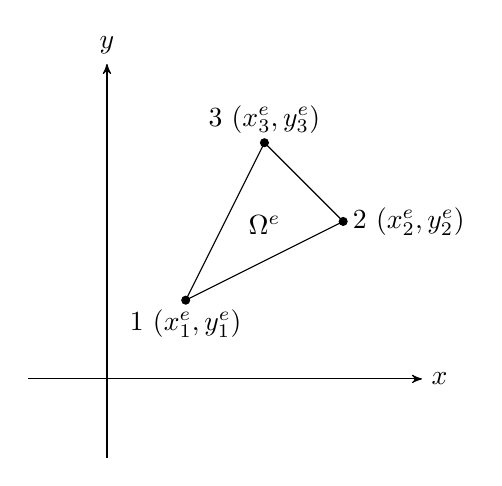
\begin{tikzpicture}[>=stealth']
            \draw[->](-1,0) -- (4,0) node[right]{$x$};
            \draw[->](0,-1) -- (0,4) node[above]{$y$};
            \filldraw [black] (1,1) circle (0.5mm);
            \filldraw [black] (3,2) circle (0.5mm);
            \filldraw [black] (2,3) circle (0.5mm);
            \draw 
                (1,1)node[below]{1 $(x^e_1, y^e_1)$} --
                (3,2)node[right]{2 $(x^e_2, y^e_2)$} --
                (2,3)node[above]{3 $(x^e_3, y^e_3)$} -- (1,1);
            \draw (2,2.2)node [below]{$\Omega^e$};
      \end{tikzpicture}
      \caption{$x$-$y$座標系}
      \label{fig:element:physical}
    \end{subfigure}
    \begin{subfigure}{0.45\columnwidth}
        \centering
        \begin{tikzpicture}[>=stealth']
            \draw[->](-1,0) -- (4,0) node[right]{$\xi$};
            \draw[->](0,-1) -- (0,4) node[above]{$\eta$};
            \draw (3,0) -- (0,3); 
            \draw (0,0) circle (0.5mm) node[below left]{1 $(0,0)$};
            \draw (3,0) circle (0.5mm) node[below]{2 $(0,1)$};
            \draw (0,3) circle (0.5mm) node[left]{3 $(1,0)$};
            \draw (1,0.8)node [above]{$\hat{\Omega}^e$};
      \end{tikzpicture}
      \caption{$\xi$-$\eta$座標系}
      \label{fig:element:natural}
    \end{subfigure}
    \caption{座標変換}
    \label{fig:element}
\end{figure}
図\ref{fig:element:physical}のような$x$-$y$座標系にある要素を図\ref{fig:element:natural}に示す
$\xi$-$\eta$座標系に座標変換する.
この変換は1次関数で表すことができるので.
\begin{align}
    x = \alpha + \beta\xi + \gamma\eta
\end{align}
と表される. 
これに図\ref{fig:element}の対応関係から係数$\alpha,\,\beta,\,\gamma$の値が以下の通りとなる.
\begin{align}
    \alpha = x^e_1,\quad 
    \beta = x^e_2 -  x^e_1,\quad 
    \gamma = x^e_3 - x^e_1
\end{align}
行列を用いて表記すると以下の式が得られる.
\begin{align}
    x    =
    \begin{bmatrix}
        1 & \xi & \eta
    \end{bmatrix}
    \begin{bmatrix}
        1 & 0 & 0 \\
        -1 & 1 & 0 \\
        -1 & 0 & 1
    \end{bmatrix}
    \label{eq:transformation:x:matrix}
\end{align}
$\xi$-$\eta$形状関数を考える. 
図\ref{fig:element:natural}から
\begin{align}
    N^e_1 = 1-\xi-\eta,\quad N^e_2 = \xi,\quad N^e_3 =\eta
\end{align}
となる. 
行列を用いて表記すると以下の式が得られる.
\begin{align}
    \begin{bmatrix}
        N^e_1 & N^e_2 & N^e_3
    \end{bmatrix}
    =
    \begin{bmatrix}
        1 & \xi & \eta
    \end{bmatrix}
    \begin{bmatrix}
        1 & 0 & 0 \\
        -1 & 1 & 0 \\
        -1 & 0 & 1
    \end{bmatrix}
\end{align}
式\eqref{eq:transformation:x:matrix}の関係から
\begin{align}
    x = 
    \begin{bmatrix}
        N^e_1 & N^e_2 & N^e_3
    \end{bmatrix}
    \begin{bmatrix}
        x^e_1 \\ x^e_2 \\ x^e_3
    \end{bmatrix}
\end{align}
となり, $y$座標の変数変換についても同様に考察すると, 以下の式が得られる.
\begin{align}
    y = 
    \begin{bmatrix}
        N^e_1 & N^e_2 & N^e_3
    \end{bmatrix}
    \begin{bmatrix}
        y^e_1 \\ y^e_2 \\ y^e_3
    \end{bmatrix}
\end{align}
ベクトル表記でまとめると
\begin{align}
    \bm{x} = \sum_{i=1}^3 N^e_i(\bm{\xi})\bm{x}^e_i. \label{eq:transformation}
\end{align}
式\eqref{eq:transformation}のヤコビ行列$\bm{J}^e$は以下の通りに求められる.
\begin{align}
    \begin{split}
        \bm{J}^e %&= \pdv{(x,y)}{(\xi,\eta)}\\
        &= 
        \begin{bmatrix}
            \pdv{x}{\xi} & \pdv{x}{\eta} \\
            \pdv{y}{\xi} & \pdv{y}{\eta} 
        \end{bmatrix}\\
        &=
        \begin{bmatrix}
            \sum_i\pdv{N^e_i}{\xi}\bm{x}^e_i & \sum_i\pdv{N^e_i}{\eta}\bm{x}^e_i
        \end{bmatrix} \\
        &=
        \begin{bmatrix}
            -\bm{x}^e_1+\bm{x}^e_2 & -\bm{x}^e_1+\bm{x}^e_3
        \end{bmatrix}
    \end{split}
\end{align}
したがってヤコビ行列の行列式$|\bm{J}^e|$は
\begin{align}
    \begin{split}
        |\bm{J}^e| &=
        \begin{vmatrix}
            -\bm{x}^e_1+\bm{x}^e_2 & -\bm{x}^e_1+\bm{x}^e_3
        \end{vmatrix} = 2|\Omega^e|.
        \label{eq:jacobian:determinant}
    \end{split}
\end{align}

次にベクトルの積分を評価する. 座標変換により積分は以下のように書き換えられる.
\begin{align}
    \int_{\Omega^e} f^eN_i^e\dd{V}
    = \int_0^1\int_0^{1-\xi}f^eN_i^e|\bm{J}^e|\dd{\eta}\dd{\xi} 
\end{align}
次に積分を領域上の被積分関数の値の重み付き和で近似すると
以下の式が得られる. $n_p$は評価点の数である.
\begin{align}
    \int_0^1\int_0^{1-\xi}f^eN_i^e|\bm{J}^e|\dd{\eta}\dd{\xi} 
    \approx 2\sum_{p=1}^{n_p}f^e(\xi_p,\eta_p)N_i^e(\xi_p,\eta_p)|\Omega^e|W_p
\end{align}
ここで式\eqref{eq:jacobian:determinant}の結果を用いた.
文献\cite{Wriggers2006}によると3次精度の場合,
評価点の位置と重みは表\ref{tab:gauss_quadrature}の通りとなる.
\begin{table}[htbp]
    \centering
    \caption{三角形要素のガウス求積}
    \label{tab:gauss_quadrature}
    \begin{tabular}{lllr}
        \hline
        $p$ & $\xi_p$ &  $\eta_p$ & $W_p$ \\ \hline
        1 & $1/3$ & $1/3$ & $-27/96$ \\
        2 & $1/5$ & $1/5$ & $25/96$ \\
        3 & $3/5$ & $1/5$ & $25/96$ \\
        4 & $1/5$ & $3/5$ & $25/96$ \\ \hline
    \end{tabular}
\end{table}


\section{計算例}
先程述べた有限要素解析を検証するために以下の問題を解く.
\begin{alignat}{4}
    \nabla^2 u + 2\pi^2\sin(\pi x)\sin(\pi y) &= 0 &\quad& \mathrm{in}\, (0\leq x \leq 1, 0\leq y\leq 1) \\
    u &= 0 &\quad& \mathrm{on\,boundary}
\end{alignat}
厳密解は
\begin{align}
    u = \sin(\pi x)\sin(\pi y).
\end{align}
要素を短辺の長さが0.1の直角二等辺三角形で分割し, 計算を行った.
結果を図\ref{fig:visualization}に示す.
\begin{figure}[htbp]
    \centering
    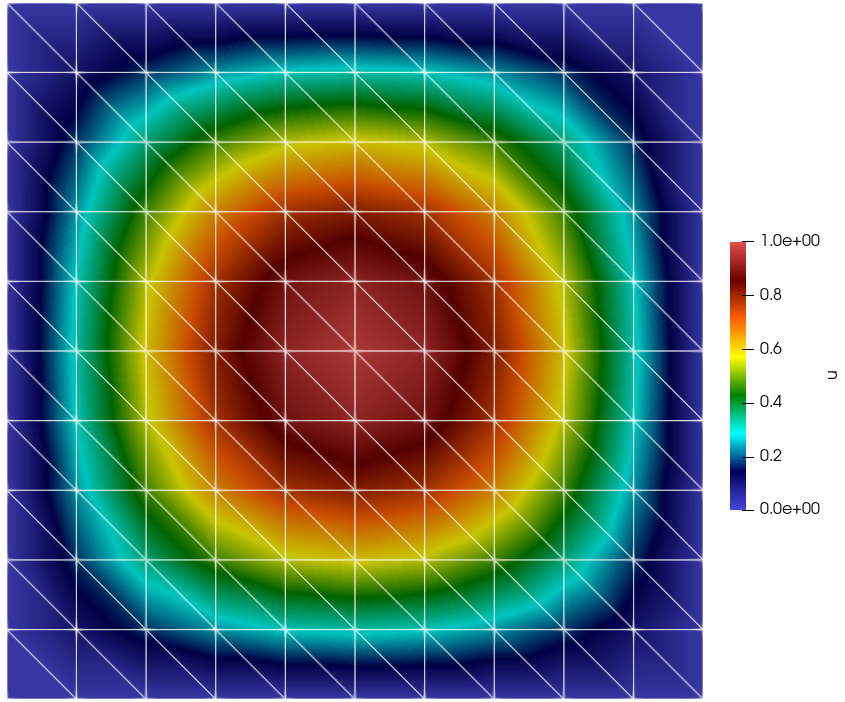
\includegraphics[width=7cm]{visualization.png}
    \caption{計算結果}
    \label{fig:visualization}
\end{figure}
計算結果が解析解と定性的に一致しており, 正しく問題を解くことができたと考えられる.

\begin{thebibliography}{9}
    \bibitem{Larson2013} Mats G. Larson and Fredrik Bengzon, ``The Finite Element Method: Theory,  Implementation,  and Applications'', Springer Berlin Heidelberg, \url{https://doi.org/10.1007/978-3-642-33287-6}, pp. 71--112, 2013
    \bibitem{Wriggers2006} Peter Wriggers, ``Computational Contact Mechanics'', Springer Berlin Heidelberg, \url{https://doi.org/10.1007/978-3-540-32609-0}, pp.473--476, 2006 
\end{thebibliography}
\end{document}